%% FullCourse_10Lecs -- Lecture 7, Act 5 (MEASURE, part 2/2): Applications & Validation
%% ch14 rebuild (2026-07-07), per Lec07_ch14_Rebuild_Plan_2026-07-07.md.
%% Reused frames copied verbatim (with renumbered cross-references) from
%%   archive_pre_split/pre_ch14_rebuild_2026-07-07/Lec07_T4_Textual_Analysis.tex (applications, validation, disclosure)
%%   archive_pre_split/pre_ch14_rebuild_2026-07-07/Lec07_T3b_Limits_Measurement.tex (AI-exposure instrument arc,
%%     "When NOT to Use an LLM Rater", grounded-generation close; "Next Step: Extending
%%     the Brain" merged into the closing bridge)
%% New frames follow chapter14 sec. 14.6.2-4 + 14.7: cosine-as-economic-variable,
%% generated-regressor problem, zero-shot classification, three starter paths,
%% thesis frame "Identification precedes measurement", map reprise (k=0).

%% Shared preamble for the FullCourse_10Lecs topic decks.
%%
%% Each topic .tex \input's this file, then defines its own \title, \date
%% override (if any), \graphicspath, and \begin{document}.
%%
%% Reconstructed verbatim from the inlined copy preserved in
%% Lec10_Case_Studies/Lec10_T8_Case6_DeepRamsey.tex (lines 23-190), which is
%% explicitly annotated there as "from ../shared_preamble.tex, copied verbatim".
%% Base preamble matches MiniCourse_8hr/Slides/shared_preamble.tex; this version
%% additionally provides \sectiondivider, the conceptbox/cautionbox/examplebox/
%% takeawaybox tcolorboxes, and \compacttables used across the split decks.

\documentclass[10pt,english,aspectratio=169]{beamer}

\usepackage{ae,aecompl}
\usepackage[T1]{fontenc}
\usepackage{textcomp}
\usepackage[utf8]{inputenc}
\usepackage{babel}
\usepackage{datetime2}

\setcounter{secnumdepth}{3}
\setcounter{tocdepth}{3}

\usepackage{amsmath, amssymb, amsthm, graphicx}
\usepackage{booktabs, multirow}
\usepackage{tikz}
\usepackage{pgfplots}
\pgfplotsset{compat=1.16}
\usepackage[most]{tcolorbox}
\tcbuselibrary{skins, breakable, theorems}
\usepackage{listings}
\usepackage{xcolor}

\lstset{
  basicstyle=\ttfamily\small,
  keywordstyle=\color{blue!80!black}\bfseries,
  commentstyle=\color{green!50!black}\itshape,
  stringstyle=\color{orange!80!black},
  backgroundcolor=\color{gray!8},
  frame=single,
  rulecolor=\color{gray!40},
  breaklines=true,
  showstringspaces=false,
  numbers=none,
}

\lstdefinestyle{pythonstyle}{
    language=Python,
    basicstyle=\ttfamily\footnotesize,
    keywordstyle=\color{blue!80!black}\bfseries,
    commentstyle=\color{green!50!black}\itshape,
    stringstyle=\color{orange!80!black},
    frame=single,
    breaklines=true,
    showstringspaces=false,
    numbers=left,
    numbersep=5pt,
    numberstyle=\tiny\color{gray},
    backgroundcolor=\color{gray!8},
    rulecolor=\color{gray!40}
}

\ifx\hypersetup\undefined
  \AtBeginDocument{%
    \hypersetup{bookmarks=false,breaklinks=true,pdfborder={0 0 0},colorlinks=true,
      linkcolor=DarkText,urlcolor=RedTitle}%
  }
\else
  \hypersetup{bookmarks=false,breaklinks=true,pdfborder={0 0 0},colorlinks=true,
    linkcolor=DarkText,urlcolor=RedTitle}%
\fi

\makeatletter
\newcommand\makebeamertitle{%
  \begin{frame}[plain]
    \vspace*{1.0cm}
    \centering
    {\usebeamerfont{title}\usebeamercolor[fg]{title}\inserttitle\par}
    \vspace{1.0cm}
    {\usebeamerfont{author}\usebeamercolor[fg]{author}\insertauthor\par}
    \vspace{0.2cm}
    {\usebeamerfont{date}\usebeamercolor[fg]{date}\insertdate\par}
  \end{frame}}%
\AtBeginDocument{%
  \let\origtableofcontents=\tableofcontents
  \def\tableofcontents{\@ifnextchar[{\origtableofcontents}{\gobbletableofcontents}}
  \def\gobbletableofcontents#1{\origtableofcontents}%
}

\usetheme{metropolis}
\usefonttheme{professionalfonts}

\definecolor{LightGray}{RGB}{230,230,230}
\definecolor{RedTitle}{RGB}{0,0,200}
\definecolor{VeryLightGray}{RGB}{245,245,245}
\definecolor{DarkText}{RGB}{0,0,0}

\setbeamercolor{background canvas}{bg=white}
\setbeamercolor{title}{fg=RedTitle}
\setbeamercolor{author}{fg=DarkText}
\setbeamercolor{date}{fg=DarkText}
\setbeamercolor{frametitle}{bg=VeryLightGray,fg=DarkText}
\setbeamercolor{normal text}{fg=DarkText}
\setbeamerfont{title}{size=\large}

\setbeamersize{text margin left=5mm, text margin right=5mm}
\addtobeamertemplate{frametitle}{}{\vspace{-0.5em}}
\newcommand{\reducevspace}{\vspace{-0.5cm}}

% Shared section divider and box styles for split topic decks.
\newcommand{\sectiondivider}[2]{%
\begin{frame}[plain,noframenumbering]
\begin{center}
\vfill
{\Large\textbf{#1}\par}
\vspace{0.35cm}
{\normalsize #2\par}
\vfill
\end{center}
\end{frame}
}

\newtcolorbox{conceptbox}[1][]{
  colback=blue!3,
  colframe=RedTitle!55,
  boxrule=0.35mm,
  arc=1mm,
  left=2mm,
  right=2mm,
  top=1mm,
  bottom=1mm,
  #1
}
\newtcolorbox{cautionbox}[1][]{
  colback=red!3,
  colframe=red!50!black,
  boxrule=0.35mm,
  arc=1mm,
  left=2mm,
  right=2mm,
  top=1mm,
  bottom=1mm,
  #1
}
\newtcolorbox{examplebox}[1][]{
  colback=green!3,
  colframe=green!45!black,
  boxrule=0.35mm,
  arc=1mm,
  left=2mm,
  right=2mm,
  top=1mm,
  bottom=1mm,
  #1
}
\newtcolorbox{takeawaybox}[1][]{
  colback=VeryLightGray,
  colframe=RedTitle!55,
  boxrule=0.35mm,
  arc=1mm,
  left=2mm,
  right=2mm,
  top=1mm,
  bottom=1mm,
  #1
}
\newcommand{\compacttables}{\renewcommand{\arraystretch}{1.15}}

\setbeamertemplate{navigation symbols}{}
\setbeamertemplate{footline}{%
  \hfill%
  \usebeamercolor[fg]{page number in head/foot}%
  \usebeamerfont{page number in head/foot}%
  \insertframenumber\,/\,\inserttotalframenumber\kern1em\vskip2pt%
}

\makeatother

\author{Zhigang Feng}
% "date with time": compile timestamp so each build is identifiable.
\date{\today\ \DTMcurrenttime}


\metroset{sectionpage=none}

\graphicspath{{./pic/}{../../MiniCourse_8hr/Slides/Module3_LLM_Text/pic/}{../}}

\usetikzlibrary{arrows.meta, positioning, shapes.geometric, fit, backgrounds}

%% Lec07 shared MAP slide: "one map, five acts" recurring diagram.
%% Adapted from ../Lec09_Agentic_AI/lec09_map.tex (\LecNineMap -> \LecSevenMap).
%% Input this file AFTER ../shared_preamble.tex (needs RedTitle, VeryLightGray)
%% and call \LecSevenMap{k} inside a frame, where k in {1..5} highlights the
%% current act ("you are here") and k = 0 renders the closing reprise with all
%% five acts complete (used by T5b's closing frame).
%% Filename deliberately does not match the build glob Lec*_T*.tex, so the
%% build script never tries to compile it standalone.

\newcommand{\LecSevenMap}[1]{%
% Precompute per-box style selectors; TikZ option lists are comma-split before
% TeX conditionals run, so \ifnum must not sit inside a [...] options list.
\ifnum#1=0
  \tikzset{lecmapa/.style={lecmapdone}, lecmapb/.style={lecmapdone},
           lecmapc/.style={lecmapdone}, lecmapd/.style={lecmapdone},
           lecmape/.style={lecmapdone}}%
\else
  \tikzset{lecmapa/.style={}, lecmapb/.style={}, lecmapc/.style={},
           lecmapd/.style={}, lecmape/.style={}}%
  \ifnum#1=1 \tikzset{lecmapa/.style={lecmapcur}}\fi
  \ifnum#1=2 \tikzset{lecmapb/.style={lecmapcur}}\fi
  \ifnum#1=3 \tikzset{lecmapc/.style={lecmapcur}}\fi
  \ifnum#1=4 \tikzset{lecmapd/.style={lecmapcur}}\fi
  \ifnum#1=5 \tikzset{lecmape/.style={lecmapcur}}\fi
\fi
\begin{center}
\begin{tikzpicture}[
    act/.style={rectangle, rounded corners, draw=black!60, fill=VeryLightGray,
        minimum width=2.6cm, minimum height=0.92cm, text width=2.5cm,
        align=center, font=\scriptsize, text=DarkText},
    lecmapcur/.style={draw=RedTitle, very thick, fill=orange!20},
    lecmapdone/.style={draw=green!45!black, thick, fill=green!10},
    q/.style={font=\tiny\itshape, text width=2.7cm, align=center, text=black!70},
    sat/.style={rectangle, rounded corners, draw=black!45, dashed, fill=white,
        text width=5.0cm, align=center, font=\tiny, text=black!70,
        minimum height=0.5cm},
    barlab/.style={font=\tiny\bfseries, text=black!60},
    arr/.style={-{Stealth[length=2mm]}, thick, gray!60}
]
    % --- five act boxes ---
    \node[act, lecmapa] (a1) at (0,0)
        {\textbf{7.1 FRAME}\\ \tiny text as measurement};
    \node[act, lecmapb] (a2) at (2.85,0)
        {\textbf{7.2 REPRESENT}\\ \tiny tokens $\to$ vectors};
    \node[act, lecmapc] (a3) at (5.7,0)
        {\textbf{7.3 ATTEND}\\ \tiny attention \& Transformer};
    \node[act, lecmapd] (a4) at (8.55,0)
        {\textbf{7.4 PRETRAIN}\\ \tiny LMs \& alignment};
    \node[act, lecmape] (a5) at (11.4,0)
        {\textbf{7.5 MEASURE}\\ \tiny limits, apps, validation};
    \draw[arr] (a1) -- (a2);
    \draw[arr] (a2) -- (a3);
    \draw[arr] (a3) -- (a4);
    \draw[arr] (a4) -- (a5);
    % --- the student question each act answers ---
    \node[q] at (0,-0.82)    {what generates\\ this text?};
    \node[q] at (2.85,-0.82) {how do we turn it\\ into numbers?};
    \node[q] at (5.7,-0.82)  {how does context\\ get encoded?};
    \node[q] at (8.55,-0.82) {where does a pretrained\\ model come from?};
    \node[q] at (11.4,-0.82) {is my measure valid ---\\ and defensible?};
    % --- "you are here" marker above the current act ---
    \ifnum#1=1 \node[font=\scriptsize\bfseries, text=RedTitle] at (0,0.95)
        {you are here\ $\blacktriangledown$};\fi
    \ifnum#1=2 \node[font=\scriptsize\bfseries, text=RedTitle] at (2.85,0.95)
        {you are here\ $\blacktriangledown$};\fi
    \ifnum#1=3 \node[font=\scriptsize\bfseries, text=RedTitle] at (5.7,0.95)
        {you are here\ $\blacktriangledown$};\fi
    \ifnum#1=4 \node[font=\scriptsize\bfseries, text=RedTitle] at (8.55,0.95)
        {you are here\ $\blacktriangledown$};\fi
    \ifnum#1=5 \node[font=\scriptsize\bfseries, text=RedTitle] at (11.4,0.95)
        {you are here\ $\blacktriangledown$};\fi
    \ifnum#1=0 \node[font=\scriptsize\bfseries, text=green!45!black] at (5.7,0.95)
        {all five acts complete};\fi
    % --- bottom band: the measurement sandwich ---
    \fill[blue!10]   (-1.3,-1.55) rectangle (1.40,-1.22);
    \fill[green!10]  (1.65,-1.55) rectangle (9.85,-1.22);
    \fill[orange!15] (10.1,-1.55) rectangle (12.7,-1.22);
    \node[barlab] at (0.05,-1.385) {WHY TEXT = MEASUREMENT};
    \node[barlab] at (5.75,-1.385) {HOW THE MACHINE READS TEXT};
    \node[barlab] at (11.4,-1.385) {MEASURE, VALIDATE, DISCLOSE};
    % --- the recurring spine (text DGP), printed under the band ---
    \node[font=\tiny\itshape, text=black!60] at (5.7,-1.83)
        {the spine:\ \ $x_i = g(s_i,\,a_i,\,c_i)+\varepsilon_i
         \;\longrightarrow\; m(x_i)
         \;\longrightarrow\; y_i = \beta\,m(x_i)+\gamma z_i+u_i$};
    % --- dashed satellites: the neighbouring lectures ---
    \node[sat] at (2.0,-2.42)
        {\textit{before 7.1:} Lec03--04 gave you neural nets, backprop \& PyTorch --- Lec07 teaches them to read};
    \node[sat] at (9.8,-2.42)
        {\textit{after 7.5:} Lec08 RAG (grounded memory) $\to$ Lec09 agents (grounded action) $\to$ Lec10 cases};
\end{tikzpicture}
\end{center}
}


\title[AI for Econ Research]{AI for Economic Research: Dynamic Models, Language, and Agents\\
Lecture 7.5b: Applications and Validation}

\begin{document}

\makebeamertitle

%=============================================================================
\begin{frame}{Lecture 7 in One Map}
\LecSevenMap{5}
\medskip
\textit{\footnotesize Route: three featured cases $\to$ the 2024--26 frontier $\to$ embeddings as regression variables $\to$ the AI-exposure cautionary tale $\to$ the validation workflow $\to$ the thesis (part 2/2 of MEASURE, and the close of Lecture 7).}
\end{frame}

%=============================================================================
\section{Three Featured Cases}
\sectiondivider{Three Featured Cases}{Word2Vec forecasting, TF-IDF exposure, domain encoders --- Thread A and B pay off}

\begin{frame}{Three Featured Case Studies}
\begin{enumerate}
\item \textbf{ECB Word2Prices} (Araujo, Bokan, Comazzi \& Lenza, 2025)
   \begin{itemize}
       \item Word2Vec on ECB statements + BVAR for inflation forecasting
   \end{itemize}

\medskip
\item \textbf{Patents and Worker Exposure} (Kogan et al., 2019)
   \begin{itemize}
       \item TF-IDF + cosine similarity between patents and occupational tasks
   \end{itemize}

\medskip
\item \textbf{Central Bank Sentiment with BERT} (Pfeifer \& Marohl, 2023; Ganguli et al., 2024)
   \begin{itemize}
       \item Fine-tuned RoBERTa for sentiment toward different economic agents
       \item PaECTER patent embeddings for innovation dynamics
   \end{itemize}
\end{enumerate}

\medskip
After the three deep dives: the 2024--26 frontier, then the tools that turn embeddings into regression variables --- and the validation discipline that makes any of it publishable.
\end{frame}

\begin{frame}{Case 1 --- ECB Word2Prices: Setup}
\textbf{Araujo, Bokan, Comazzi \& Lenza (2025), ECB WP No.\ 3047}

\medskip
\begin{itemize}
\item \textbf{Question:} can embeddings of ECB communications improve euro-area inflation forecasting?

\medskip
\item \textbf{Data:}
\begin{itemize}
    \item ECB press conference introductory statements, 2002Q1--2023Q4
    \item Target: HICPx (core inflation), monthly $\rightarrow$ quarterly
\end{itemize}

\medskip
\item \textbf{Method:}
\begin{itemize}
    \item For each quarter $q$, retrain Word2Vec on the corpus available \emph{up to} $q$ (no look-ahead)
    \item Average word vectors per statement; aggregate to a quarterly text vector
    \item Stack text vector with macro variables; fit a Bayesian VAR
    \item Forecast 1--4 quarters ahead
\end{itemize}

\medskip
\item \textbf{Why this design?} Re-training quarterly avoids the look-ahead bias that plagues most LLM-based forecast exercises (T2a's caution, obeyed to the letter), while remaining computationally cheap.
\end{itemize}
\end{frame}

\begin{frame}[fragile]{Case 1 --- Python Skeleton}
\begin{lstlisting}[language=Python, basicstyle=\scriptsize\ttfamily]
# Quarterly Word2Vec retraining for ECB inflation forecasting
from gensim.models import Word2Vec
from statsmodels.tsa.api import VAR
import numpy as np

forecasts = []
for q in quarters:
    # 1. Build corpus available at quarter q (no look-ahead)
    corpus_q = [s for s in all_statements if s.date <= q]
    # 2. Train Word2Vec on the available corpus
    w2v = Word2Vec(corpus_q, vector_size=100, window=5,
                   sg=0, min_count=2, epochs=20)
    # 3. Average word vectors per statement, then per quarter
    stmt_vec = [np.mean([w2v.wv[w] for w in s if w in w2v.wv], axis=0)
                for s in corpus_q]
    text_q = aggregate_quarterly(stmt_vec, dates)
    # 4. Stack with macro variables and fit a BVAR
    Y = np.column_stack([macro_q, text_q])
    bvar = VAR(Y).fit(maxlags=4)
    # 5. Forecast 1-4 quarters ahead
    forecasts.append(bvar.forecast(Y, steps=4))
\end{lstlisting}
\end{frame}

\begin{frame}{Case 1 --- Results and Lessons}
\begin{itemize}
\item \textbf{Forecast performance:}
\begin{itemize}
    \item BVAR with Word2Vec text features outperforms a baseline AR / BVAR without text at horizons of 1--4 quarters
    \item Sentiment dictionaries (e.g.\ Loughran-McDonald) deliver only marginal gains relative to the no-text baseline
    \item Heavy LLMs (BERT, fine-tuned) can match or beat Word2Vec but are much more expensive and harder to retrain quarterly --- look-ahead bias becomes a real risk
\end{itemize}

\medskip
\item \textbf{Take-aways for empirical economists:}
\begin{itemize}
    \item ``Lighter is better'' if it lets you respect the timing structure of the forecasting exercise
    \item Frequently-retrained Word2Vec is a strong baseline before reaching for an LLM
    \item Always document: training corpus cutoff at every step, vector dimension, window, retraining frequency
\end{itemize}

\medskip
\item Replicable framework with zero GPU requirements --- ideal for grad-student empirical work.
\end{itemize}
\end{frame}

\begin{frame}{Case 2 --- Patent Text and Worker Exposure}
\textbf{Kogan, Papanikolaou, Schmidt, Seegmiller (2019, 2023)}

\medskip
\begin{itemize}
\item \textbf{Question:} how does exposure to technological innovation affect workers' earnings and employment?

\medskip
\item \textbf{Method:}
\begin{itemize}
    \item Compute TF-IDF vectors for U.S.\ patent texts and for O*NET occupational task descriptions
    \item Measure cosine similarity between each occupation and each patent
    \item Aggregate up: occupation-level technological exposure
\end{itemize}

\medskip
\item \textbf{Findings:}
\begin{itemize}
    \item High-exposure occupations experience earnings declines and reduced employment stability
    \item Effects are present for both low- and high-wage workers
\end{itemize}

\medskip
\item \textbf{Why this is in our lecture:} a textbook example of how a \emph{simple} method (TF-IDF + cosine, T2a's toolkit) on a \emph{thoughtfully chosen} corpus can answer a substantive economic question. You don't need transformers to make a contribution, but you do need a clean identification strategy.
\end{itemize}
\end{frame}

\begin{frame}{Why Generic LLMs Underperform on Financial Text}
\textbf{The vocabulary mismatch.} Generic BERT/GPT was trained on Wikipedia, web text, and books --- not on disclosure language.

\medskip
\begin{itemize}
  \item \textbf{Polarity flips.} ``Liability,'' ``aggressive,'' ``exposure'' are negative in everyday English but neutral or positive in accounting/finance. Loughran \& McDonald (2011) is the canonical correction of the older Harvard-IV-4 list.
  \medskip
  \item \textbf{Hedging language.} ``May,'' ``could,'' ``intend to'' are stop-words in generic NLP but encode legal disclosure stance in 10-K text.
  \medskip
  \item \textbf{Numbers in context.} Subword tokenizers split \texttt{1.2345} into digit tokens; without finance fine-tuning the model treats the magnitude as just another vocabulary item.
\end{itemize}

\medskip
\textbf{Two responses:} (1) train a domain-specific encoder (next slide), or (2) zero-shot prompt a frontier LLM and validate carefully (Hansen \& Kazinnik, 2023).
\end{frame}

\begin{frame}{Case 3a --- FinBERT and CentralBankRoBERTa: Two Domain Encoders}
\begin{center}
\renewcommand{\arraystretch}{1.25}
\footnotesize
\begin{tabular}{|p{2.6cm}|p{4.0cm}|p{6.4cm}|}
\hline
& \textbf{FinBERT} (Araci, 2019; Yang et al., 2020) & \textbf{CentralBankRoBERTa} (Pfeifer \& Marohl, 2023) \\ \hline
Backbone & BERT-base (12 layers, 110M params) & RoBERTa-base, fine-tuned \\ \hline
Pre-train corpus & Reuters TRC2-Financial + 10-K corpora & RoBERTa-base fine-tuned on $\sim$12k hand-labeled sentences (plus ECB/BIS pseudo-labels) \\ \hline
Task it ships for & 3-way sentiment (positive/negative/neutral) on financial sentences & Agent-specific sentiment: stance toward five macro agents (households, firms, financial sector, government, central bank) \\ \hline
Headline result & Beats LSTM/dictionary baselines on Financial PhraseBank & Agent-specific scores predict regional inflation \& employment better than ``hawkish/dovish'' \\ \hline
When to reach for it & Fast firm-level sentiment at scale & Central-bank communication studies \\ \hline
\end{tabular}
\end{center}

\medskip
\textbf{Both are fine-tuned BERTs} --- the architecture is Act 3; the pretraining/fine-tuning recipe is Act 4 (base $\to$ DAPT on domain text $\to$ small labeled head). This deck cares only about \emph{using} them: load weights, feed sentences, get scores.
\end{frame}

\begin{frame}{Domain Models vs.\ Frontier LLMs: No Single Winner}
\textbf{Hansen \& Kazinnik (2023): ``GPT-4 reads Fedspeak.''} Zero-shot GPT-4 classifies FOMC sentence stance at expert-level accuracy; beats fine-tuned BERT/RoBERTa; provides human-consistent explanations.

\smallskip
\textbf{Gambacorta et al.\ (BIS WP 1215, 2024): CB-LMs.} Domain-adapted encoder beats generic BERT on FOMC stance; GPT-4 still wins on complex narrative tasks.

\smallskip
\textbf{Practical decision rule:}
\begin{itemize}\itemsep1pt
  \item \textbf{Sentence-level sentiment at scale, fixed taxonomy} $\to$ FinBERT / CentralBankRoBERTa (cheap, deterministic, citable).
  \item \textbf{Open-ended interpretation, narrative, novel category} $\to$ frontier LLM (GPT-4, Claude) with a logged prompt.
  \item \textbf{In doubt} $\to$ run both and report agreement (Cohen's $\kappa$).
\end{itemize}

\smallskip
\textit{No single model dominates --- the validation workflow (later in this deck) handles the choice. And recall T4: the frontier LLM's scores move with its version; the frozen encoder's do not.}
\end{frame}

\begin{frame}{Case 3b --- PaECTER for Patent Innovation}
\textbf{Ganguli, Lin \& Reynolds (2024), NBER WP}

\medskip
\begin{itemize}
\item \textbf{Goal:} measure innovation dynamics from patent text using transformer-based embeddings.

\medskip
\item \textbf{Model: PaECTER} (Patent Embeddings from Citation-Enhanced Transformer Representations)
\begin{itemize}
    \item Initialize from BERT-base
    \item Fine-tune on patent corpora
    \item Use citation pairs as a supervised signal during fine-tuning (related patents pulled together in embedding space)
\end{itemize}

\medskip
\item \textbf{Findings:}
\begin{itemize}
    \item Significantly more accurate similarity judgments than TF-IDF or LDA
    \item Distinguishes incremental from radical innovations
    \item Long-run trend: patents are increasingly diverging in semantic space (broader exploration)
\end{itemize}

\medskip
\item \textbf{Take-away:} fine-tuned transformer embeddings give a richer, citation-aware view of technological evolution than purely text-based or count-based methods.
\end{itemize}
\end{frame}

%=============================================================================
\section{The 2024--26 Frontier}
\sectiondivider{The 2024--26 Frontier}{Central-bank communication and asset pricing move to LLM-scale}

\begin{frame}{Frontier (2024--25): LLMs for Central Bank Communication}
\begin{itemize}
\item \textbf{CB-LMs} (Gambacorta et al., BIS WP 1215, 2024)
\begin{itemize}
    \item Domain-adapted encoder retrained on 37{,}000 central bank papers + 18{,}000 speeches
    \item Outperforms generic BERT on FOMC stance classification
    \item But: GPT-4 wins on complex narrative tasks --- no single model dominates
\end{itemize}

\medskip
\item \textbf{GPT-4 for Fedspeak} (Hansen \& Kazinnik, 2023)
\begin{itemize}
    \item GPT-4 classifies FOMC statement sentences at \emph{expert-level} accuracy
    \item Outperforms fine-tuned BERT/RoBERTa; provides human-consistent explanations
    \item Zero-shot performance collapses domain-adaptation barrier for many tasks
\end{itemize}

\medskip
\item \textbf{GPT-4o on 25{,}000 FOMC Sentences} (Federal Reserve FEDS Note, December 2024)
\begin{itemize}
    \item Topic classification across 2010--2024 minutes at scale
    \item Detects ``financial stability'' discourse spikes in 2020 and 2023 banking crises
    \item LLMs reveal \emph{thematic shifts} that sentiment scores miss
\end{itemize}

\medskip
\item \textbf{74{,}882 Central Bank Documents} (Silva, Moriya \& Veyrune, IMF WP 2025/109)
\begin{itemize}
    \item 169 central banks, 1884--2025; LLM-coded stance + directional communication index
    \item Forecasts future policy rate changes; documents shift to forward-looking language
\end{itemize}
\end{itemize}
\end{frame}

\begin{frame}{Frontier (2024--25): LLMs in Asset Pricing}
\begin{itemize}
\item \textbf{Expected Returns and LLMs} (Chen, Kelly \& Xiu, NBER WP 31502, 2024)
\begin{itemize}
    \item LLM embeddings of financial news $\Rightarrow$ cross-sectional equity return prediction
    \item Substantially outperforms TF-IDF and momentum; gains largest on \emph{negation} and complex narratives --- exactly the static-embedding failure cases from T2b
    \item Evidence of slow price adjustment to information that only LLM embeddings extract
\end{itemize}

\medskip
\item \textbf{AI Asset Pricing Models} (Kelly, Kuznetsov, Malamud \& Xu, NBER WP 33351, 2025)
\begin{itemize}
    \item Transformer architecture embedded directly in the stochastic discount factor $M_{t+1}$
    \item Multi-head attention learns cross-asset dependencies from 132 stock characteristics
    \item Large reductions in pricing errors vs.\ previous ML factor models
\end{itemize}

\medskip
\item \textbf{Asset Embeddings} (Gabaix, Koijen, Richmond \& Yogo, NBER WP 33651, 2025)
\begin{itemize}
    \item Embeddings learned from \emph{investor portfolio holdings} via skip-gram (same math as T2b's Word2Vec)
    \item Arithmetic: \texttt{tech $+$ growth $-$ hardware $\approx$ software firms}
    \item GPT-4 generates economic narratives for firm clusters in the learned embedding space
\end{itemize}

\medskip
\item \textbf{Key insight:} the same transformer and embedding toolkit that encodes language can encode financial structure --- text and quantitative data are no longer separate worlds.
\end{itemize}
\end{frame}

%=============================================================================
\section{Embeddings as Regression Variables}
\sectiondivider{Embeddings as Regression Variables}{Similarity, classification --- and the standard errors they deserve}

\begin{frame}{Cosine Similarity as an Economic Variable (Thread B)}
\textbf{The most direct embedding-to-regression path: distance between documents.}
\begin{itemize}
\item $\mathrm{sim}(i,j) = \frac{\mathbf{e}_i^\top \mathbf{e}_j}{\|\mathbf{e}_i\|\,\|\mathbf{e}_j\|}$; cosine \emph{distance} $= 1-\mathrm{sim}$. Length-invariant by construction --- and that matters, because document length tracks firm size and disclosure habits.
\item \textbf{Statement-change series:} $\delta_t = 1 - \mathrm{sim}(D_{t-1}, D_t)$ across consecutive FOMC statements gives a continuous ``how much did the message change'' measure --- finer than hawk/dove labels. (Similarity tracking of consecutive Fed statements goes back to Acosta \& Meade 2015.)
\item \textbf{Interpretation discipline --- two layers of endogeneity:}
\begin{itemize}
    \item the \emph{expected} component: strip out what markets already priced, e.g.\ with high-frequency windows around the release;
    \item the \emph{structural} component: the bank may deliberately say more when conditions worsen --- $\delta_t$ then responds to the economy rather than shocking it. No embedding quality fixes that; only a design can.
\end{itemize}
\end{itemize}
\smallskip
\begin{takeawaybox}
The DGP one last time: $\delta_t$ is an $m(x)$. Whether it is a \emph{shock} or an \emph{outcome} is an identification claim about $a_t$ and $c_t$ --- not a property of the vector space.
\end{takeawaybox}
\end{frame}

\begin{frame}{Validation Caveats for Econometricians}
\begin{itemize}
\item \textbf{Cosine similarity is not innocent.} Three common confounds inflate similarity between firm/policy texts:
\begin{itemize}
    \item \textbf{Industry jargon:} firms in the same SIC code share boilerplate language
    \item \textbf{Templates:} regulatory filings re-use chunks of text verbatim
    \item \textbf{Length:} longer documents have smoother averages and look more similar
\end{itemize}

\medskip
\item \textbf{Standard tools for robustness:}
\begin{itemize}
    \item Permutation tests --- shuffle labels within an industry, check if observed similarity exceeds the within-industry baseline
    \item Residual embeddings --- subtract the industry mean before measuring similarity
    \item Bootstrap the entire pipeline (text $\rightarrow$ embedding $\rightarrow$ measurement $\rightarrow$ regression) for honest standard errors (next slide)
\end{itemize}

\medskip
\item \textbf{Dictionary methods are not innocent either.} The Loughran-McDonald (2011) finance-specific dictionary corrects mismatches in the older Harvard IV-4 list (e.g.\ ``liability'' is not negative in financial accounting).

\medskip
\item \textbf{Always validate} a sample of model outputs against human coding before scaling up.
\end{itemize}
\end{frame}

\begin{frame}{The Generated-Regressor Problem}
\textbf{Your regressor was estimated --- the second stage must know that.}
\begin{itemize}
\item An embedding similarity, a topic share, an LLM score: all are \emph{estimates}, carrying error from model choice, training data, and aggregation.
\item OLS with a noisy constructed regressor $\Rightarrow$ standard errors too small, $t$-statistics too big --- the classic two-step problem, now wearing NLP clothes.
\item Worst when the first stage is trained on little data: embeddings fit on a few hundred FOMC statements carry large estimation error into every downstream $\delta_t$.
\item \textbf{Fix: bootstrap the whole pipeline} --- resample documents, re-embed, re-aggregate, re-run the regression --- so first-stage uncertainty propagates into the reported intervals. Report pipeline-bootstrap intervals next to the naive ones.
\end{itemize}
\medskip
\begin{takeawaybox}
Rule of thumb: if deleting one year of documents would visibly move your embedding space, then second-stage standard errors without the full-pipeline bootstrap are overconfident.
\end{takeawaybox}
\end{frame}

\begin{frame}{Zero-Shot Classification: Measuring Concepts with No Training Labels}
\textbf{Describe the class in a sentence; let the geometry do the rest.}
\begin{itemize}
\item $\hat c = \arg\max_{c_k} \mathrm{sim}(\mathbf{e}_{\text{doc}}, \mathbf{e}_{c_k})$: embed the document and each class \emph{description} (``this firm faces material climate-transition risk''), assign by nearest neighbor.
\item \textbf{Why it matters for economics:} new constructs --- climate exposure, AI adoption, supply-chain geopolitical risk --- have \emph{no historical labels}. Zero-shot lets you score decades of filings \emph{backwards} with today's concept, extending Hassan-style risk measures to categories nobody coded at the time.
\item \textbf{Model choice is make-or-break:} raw BERT embeddings are anisotropic --- unrelated sentences look similar because they share frequent words. Use sentence-embedding models trained contrastively for similarity (SBERT via \texttt{sentence-transformers}, BGE, E5) --- T3b's token-vs-document distinction doing real work.
\item \textbf{Validation ladder --- all three steps, in order:}
\begin{enumerate}
    \item consistency across paraphrased class descriptions (Fleiss' $\kappa > 0.6$);
    \item accuracy on a hand-coded gold subsample --- consistency is \emph{not} correctness: a systematically wrong description can be perfectly consistent;
    \item external validity against a real economic outcome.
\end{enumerate}
\end{itemize}
\end{frame}

%=============================================================================
\section{A Cautionary Tale}
\sectiondivider{A Cautionary Tale}{The AI-exposure literature --- when the instrument is the thing it measures}

\begin{frame}{The Literature's Question: How Exposed Is Each Job to AI?}
\begin{itemize}
\item \textbf{The measurement problem:} map $\sim$19{,}000 O*NET tasks (or $\sim$900 SOC occupations) to a numeric \emph{AI exposure} score that can be regressed on wages, employment, and county outcomes.

\medskip
\item \textbf{Two pre-LLM generations of measures:}
\begin{enumerate}
\item \textbf{Felten, Raj, Seamans (2018, 2021)} --- AI Occupational Exposure index (AIOE). Link AI benchmark progress (image recognition, translation, $\ldots$) to O*NET ability requirements. \emph{Mechanical mapping; human raters set the abilities.}
\item \textbf{Webb (2020)} --- text overlap of AI patent abstracts with O*NET task descriptions. \emph{No raters at all --- pure TF-IDF.}
\end{enumerate}

\medskip
\item Both treat the measurement instrument as \textbf{fixed and inspectable}. A re-run next year produces the same numbers.

\medskip
\item \textbf{Economist's framing:} exposure is a \emph{measurement-error} question, not a CS question. The next slide shows what changes when the instrument is itself an LLM.
\end{itemize}
\end{frame}

\begin{frame}{Three Generations of AI-Exposure Instruments --- Compared}
\textbf{Same target (occupation-level exposure score), three very different instruments:}

\medskip
\begin{center}
\renewcommand{\arraystretch}{1.25}
\footnotesize
\begin{tabular}{|p{2.4cm}|p{3.2cm}|p{3.2cm}|p{3.2cm}|}
\hline
& \textbf{Felten, Raj, Seamans (2018, 2021)} & \textbf{Webb (2020)} & \textbf{Eloundou et al.\ (2023)} \\
\hline
Instrument & Hand-curated map: AI benchmark $\to$ O*NET ability & TF-IDF cosine: AI patent abstracts $\to$ O*NET tasks & Single LLM call: GPT-4 rates each task on 4-level rubric \\
\hline
Cost per refresh & High (human raters, weeks) & Low (re-tokenize, rerun) & Low per call; high per provider switch \\
\hline
Stability across reruns & Identical (deterministic mapping) & Identical (deterministic) & \textbf{Stochastic}; different provider $=$ different score \\
\hline
Validity assumption & Benchmark progress proxies real capability & AI patent text proxies AI capability & The LLM is a calibrated rater \\
\hline
Auditable by economist? & Yes (rater notes) & Yes (read the patent and the task) & Partially (rationale text); not the model weights \\
\hline
Failure mode & Benchmarks lag the frontier & Patent corpus is noisy & Version drift, hallucination, prompt sensitivity \\
\hline
\end{tabular}
\end{center}

\medskip
\textbf{The structural shift.} Felten and Webb treat the instrument as a \emph{document}; Eloundou treats it as a \emph{model call}. Documents do not drift. Model calls do --- which is what the next two frames quantify.
\end{frame}

\begin{frame}{The LLM-as-Rater Turn: Eloundou et al.\ (2023)}
\begin{itemize}
\item \textbf{Eloundou, Manning, Mishkin, Rock (2023, ``GPTs are GPTs'')} --- the first paper to use \textbf{GPT-4 itself} as the rater on the O*NET task list.

\medskip
\item \textbf{Rubric (per task):}
\begin{itemize}
\item \textbf{E0} --- no LLM speedup.
\item \textbf{E1} --- direct LLM access reduces task time by $\ge 50\%$.
\item \textbf{E2} --- speedup achievable with LLM-powered software built atop the model.
\end{itemize}

\medskip
\item \textbf{Procedure:} prompt GPT-4 with a task description, ask it to classify, repeat for $\sim$19k tasks, average within occupation $\to$ exposure score.

\medskip
\item Quickly adopted as the \emph{default} exposure measure --- Acemoglu (2024), IMF (2024), BIS, and many follow-ups all rebuild on this LLM-rated input.

\medskip
\item \textbf{The instrument is now the same kind of model as the subject of the research} --- and as T5a established, that instrument is stochastic, hallucination-prone, and version-drifting.
\end{itemize}
\end{frame}

\begin{frame}{Replication: Yin, Vu, Persico (NBER 35110, 2026)}
\begin{columns}[T]
\column{0.50\textwidth}
\textbf{Design --- only the LLM changes:}
\begin{itemize}
\item Same Eloundou (2023) prompt and task list (18{,}797 O*NET tasks, $\sim$900 occupations).
\item Three frontier 2026 annotators: \textbf{ChatGPT-5}, \textbf{Claude 4.5}, \textbf{Gemini 2.5}.
\item Identical decoding (low temperature, deterministic where supported); identical few-shot examples; identical aggregation to occupation-level $E_1$ means.
\item Plug the resulting exposure scores into the same downstream difference-in-differences regressions used by the labor-AI literature.
\end{itemize}

\column{0.46\textwidth}
\begin{center}
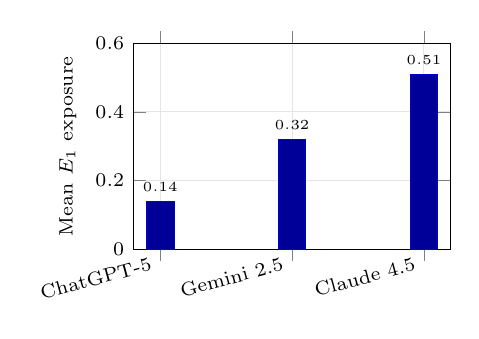
\begin{tikzpicture}
\begin{axis}[
  width=5.6cm, height=4.2cm,
  ybar,
  bar width=10pt,
  ymin=0, ymax=0.6,
  ylabel={Mean $E_1$ exposure},
  symbolic x coords={ChatGPT-5, Gemini 2.5, Claude 4.5},
  xtick=data,
  xticklabel style={font=\scriptsize, rotate=15, anchor=east},
  ytick={0,0.2,0.4,0.6},
  grid=major,
  grid style={gray!20},
  tick label style={font=\scriptsize},
  label style={font=\scriptsize},
  nodes near coords,
  nodes near coords style={font=\tiny},
]
\addplot[fill=blue!60!black, draw=blue!80!black] coordinates {
  (ChatGPT-5, 0.14)
  (Gemini 2.5, 0.32)
  (Claude 4.5, 0.51)
};
\end{axis}
\end{tikzpicture}\\
{\footnotesize Same prompt, same tasks --- 3.6$\times$ divergence in mean exposure.}
\end{center}

\smallskip
\begin{itemize}
\item \scriptsize Pairwise agreement: \textbf{56.9\%}, Cohen's $\kappa$ as low as \textbf{0.36}.
\item \scriptsize Individual DiD coefficient varies \textbf{2.4$\times$} across annotators.
\item \scriptsize County-level estimate \textbf{flips sign} (significant negative $\to$ insignificant positive).
\end{itemize}
\end{columns}

\smallskip
\textbf{What 0.36 means} (Landis--Koch benchmarks): $<\!0.20$ slight, $0.21$--$0.40$ \emph{fair}, $0.41$--$0.60$ moderate, $0.61$--$0.80$ substantial, $0.81$--$1.00$ almost perfect. Publication-grade hand-coding aims for $\kappa \ge 0.75$.
\end{frame}

\begin{frame}{Attitude in the Literature: LLMs Are Not Static Instruments}
\begin{itemize}
\item \textbf{The error is non-classical:} disagreement concentrates on tasks near the rubric boundary --- the high-exposure tasks the regressor cares about. Errors correlate with the regressor.

\medskip
\item Yin et al.: \emph{``the risks of treating evolving LLMs as static instruments.''} A paper rated with GPT-4 in 2023 cannot be re-run in 2026 and get the same labels.

\medskip
\item \textbf{Each T5a limit $\to$ a measurement consequence:}
\begin{itemize}
\item \emph{Sampling stochasticity} $\to$ set $\tau = 0$ and report it.
\item \emph{Hallucination / mis-calibration} $\to$ ensemble across models, report Cohen's $\kappa$.
\item \emph{Version drift} $\to$ pin the snapshot; treat \emph{prompt + model + seed} as one instrument.
\end{itemize}

\medskip
\item \textbf{Emerging best practice:} pre-register prompt + model + decoding; use multiple frontier annotators and report between-model agreement; audit against a hand-coded gold standard; report inter-annotator sensitivity, not a single point estimate.

\medskip
\item \textbf{Takeaway:} the LLM is a measurement instrument --- calibrate, version, and disclose.
\end{itemize}
\end{frame}

\begin{frame}{When NOT to Use an LLM Rater --- A Decision Rule}
\textbf{Pearson 0.6 from 50 lines of \texttt{re.findall} is a real signal.} The LLM rater must clear a meaningful bar to justify its cost.

\medskip
\small
\textbf{A defensible workflow before reaching for an LLM:}
\begin{enumerate}\itemsep1pt
  \item \textbf{Hand-code 100--200 task gold standard} (you, an RA, two coders for $\kappa$).
  \item \textbf{Fit a simple baseline} --- TF-IDF + logistic regression, or a keyword rule with handful of features. Report $\kappa$ vs.\ gold.
  \item \textbf{Run the LLM in parallel.} Compute $\kappa$(LLM, gold) and $\kappa$(LLM, baseline).
  \item \textbf{Decide:}
  \begin{itemize}\itemsep0pt
    \item $\kappa$(LLM, gold) $\ge 0.75$ \emph{and} substantially $>$ $\kappa$(baseline, gold) $\Rightarrow$ LLM is validated; use it, disclose model + prompt.
    \item $\kappa$(LLM, gold) $< 0.60$ or $\approx \kappa$(baseline) $\Rightarrow$ ship the baseline; LLM doesn't earn the version-drift risk.
    \item Between $0.60$ and $0.75$ $\Rightarrow$ ensemble (LLM + baseline + tie-break by hand on disagreements).
  \end{itemize}
\end{enumerate}

\medskip
\textit{The LLM is one instrument among many, not a default. The Yin--Vu--Persico replication shows what you risk by skipping the audition.}
\end{frame}

\begin{frame}{The Application Zoo, Organized by Econometric Role}
\textbf{The same text can play three very different roles. Pick the representation to match the role.}
\medskip

\begin{center}
\renewcommand{\arraystretch}{1.25}
\scriptsize
\begin{tabular}{|p{3.2cm}|p{3.7cm}|p{3.5cm}|p{3.2cm}|}
\hline
\textbf{Paper} & \textbf{Signal (regressor $m(x_i)$)} & \textbf{Outcome (behavior $y$)} & \textbf{Instrument / shock} \\
\hline
Baker--Bloom--Davis (2016) & Newspaper keyword EPU $\to$ VAR & --- & EPU surprises \\
\hline
Hoberg \& Phillips (2016) & 10-K TF-IDF cosine $\to$ product-market similarity & --- & --- \\
\hline
Hassan et al.\ (2019) & Bigram firm-level political risk $\to$ investment regression & --- & Quarterly call shocks \\
\hline
Li et al.\ (2021) & W2V on earnings calls $\to$ 5 culture dimensions & --- & --- \\
\hline
Lopez-Lira \& Tang (2023) & ChatGPT zero-shot sentiment on headlines $\to$ next-day returns & --- & --- \\
\hline
Hansen--McMahon--Prat (2018) & LDA topics & Committee speech change after transparency reform & 1993 reform date \\
\hline
Hartley (2025) & LLM-reconstructed EPU (19th c., OCR) & --- & War-news shocks \\
\hline
\end{tabular}
\end{center}

\smallskip
\footnotesize
\begin{itemize}\itemsep0pt
\item \emph{Signal column dominates the literature} --- it's the easiest role and the loudest result.
\item \emph{Outcome} requires a behavior to be \emph{caused} by something else; harder but cleaner identification.
\item \emph{Instrument / shock} use needs the exclusion restriction to survive the prompt/fine-tuning recipe --- document it.
\item \textbf{Representation/role pairing.} Measurement (signal) $\to$ transparent (TF-IDF, dictionaries); behavior $\to$ contextual embeddings; instrument $\to$ frozen-snapshot LLM with archived prompt. (Thread A closes: Hartley's GPT-4 back-extension of EPU to the 19th century --- the dictionary baseline and the frontier model, joined.)
\end{itemize}
\end{frame}

%=============================================================================
\section{Validation and Disclosure}
\sectiondivider{Validation and Disclosure}{The workflow that makes a text measure publishable}

\begin{frame}{A Six-Step Workflow for LLM-Assisted Measurement}
\begin{enumerate}
\item \textbf{Pre-alignment.} Hand-code 100--200 examples; iterate on the prompt or fine-tuning recipe until you reach acceptable agreement.
\medskip
\item \textbf{Full annotation.} Run the model on the entire sample with a frozen prompt and a frozen model version.
\medskip
\item \textbf{Gold-standard audit.} Blind-code 10\% of the sample and compute Cohen's $\kappa$ (publication threshold $\kappa \ge 0.75$).
\medskip
\item \textbf{Category-level reporting.} Don't just report overall accuracy; show the confusion matrix by class. Minority classes are often where models fail silently.
\medskip
\item \textbf{External validity check.} Link the text-derived measure to a real economic outcome (returns, investment, employment) before treating it as a measurement.
\medskip
\item \textbf{Disclosure.} Report prompt, model version, temperature ($\tau = 0$), date, all preprocessing, and provide code. Reproducibility is essential when the model behind the API can change without notice.
\end{enumerate}
\end{frame}

\begin{frame}{Worked Example: Applying the Workflow to FOMC Sentiment}
\textbf{Imagined paper:} ``GPT-4 sentiment on FOMC statements predicts 10-year yields.''

\medskip
\begin{center}
\renewcommand{\arraystretch}{1.2}
\footnotesize
\begin{tabular}{|p{2.4cm}|p{4.0cm}|p{6.6cm}|}
\hline
\textbf{Step} & \textbf{What you do} & \textbf{What goes in the appendix} \\ \hline
1. Pre-align & Hand-code 200 sentences hawk/dove/neutral & Prompt v3 (frozen); $\kappa$ vs.\ author = 0.81 \\ \hline
2. Annotate & GPT-4-2024-06-13, $\tau=0$, full corpus & Cost, runtime, retries, sha256 of inputs \\ \hline
3. Gold audit & Blind-code 10\% by RA & $\kappa = 0.78$ overall; 0.62 on ``neutral'' \\ \hline
4. By-class & Confusion matrix & Hawkish recall 0.91; neutral recall 0.66 (flagged) \\ \hline
5. External validity & Predict $\Delta y_{10}$ at FOMC dates & $\hat\beta = 4.2$ bp per unit, $t = 3.1$ \\ \hline
6. Disclose & Prompt + code on Zenodo & DOI, model card, replication run-time \\ \hline
\end{tabular}
\end{center}

\medskip
\textbf{LLM-as-judge connection.} A second LLM as a \texttt{cross-checker}: same input, different prompt, flag disagreements for human review --- the same construction-to-coefficient logic used in the AI-exposure autopsy above, and a preview of Lec09's sub-agent patterns.
\end{frame}

\begin{frame}{Disclosure Norms for AI-Assisted Empirical Work}
\footnotesize
\textbf{Minimum reproducibility package.}
\begin{itemize}\itemsep1pt
  \item \textbf{Model identity.} Provider, model name, exact version string, call date.
  \item \textbf{Prompt(s).} Frozen text in a versioned file; not paraphrased in the paper.
  \item \textbf{Sampling parameters.} Temperature, top-$p$, max tokens, seed if available.
  \item \textbf{Inputs.} sha256 of every input file; document any preprocessing.
  \item \textbf{Outputs.} Raw model outputs preserved \emph{before} any post-processing.
  \item \textbf{Code.} End-to-end script with retry logic and the exact API client version.
\end{itemize}

\smallskip
\begin{takeawaybox}
\textbf{The auditable-call triple:} $\tau = 0$ $+$ fixed seed $+$ SHA-256 of every input, with raw outputs archived. One reproducible instrument, one line in the appendix.
\end{takeawaybox}

\smallskip
\textbf{AEA policy.} The October 2024 Data and Code Availability update explicitly covers AI-assisted analysis: report when an LLM was used, for what step, and provide artifacts that let a reader reproduce the result given the same model.

\smallskip
\textbf{IRB and proprietary text.} Survey transcripts, internal memos, and clinical text often cannot be sent to a hosted API. Run an open-weights model locally (T4's menu), or obtain IRB sign-off on the provider's data-handling terms.

\smallskip
\textit{The closed-source LLM is the most-changed equipment in your empirical paper. Document it like the dataset it is.}
\end{frame}

\begin{frame}{Three Starter Paths for the Macro Researcher}
\textbf{Where to begin, by application --- each a full pipeline you can defend.}
\begin{enumerate}
\item \textbf{Central-bank stance.} Domain-adapt an encoder (EconBERT for English; MacBERT $+$ DAPT on PBOC reports for Chinese) $\to$ extract \texttt{[CLS]} embeddings $\to$ compute $\delta_t$ between consecutive statements; benchmark against Romer--Romer narrative shocks as the external anchor; add a LoRA classification head on a small labeled set if you need the hawk/dove \emph{direction}.
\medskip
\item \textbf{Policy uncertainty.} Keep Baker--Bloom--Davis as the transparent, auditable baseline (Thread A's lesson); report a preprocessing specification curve (T2a); test stationarity, and separate \emph{language} breaks from \emph{economic} breaks (T2b) before the VAR.
\medskip
\item \textbf{Nowcasting.} LDA topic shares or embedding principal components as additional factors in the standard nowcast regression --- the text block enters exactly like any other factor; but bootstrap the whole text pipeline for the standard errors (this deck).
\end{enumerate}
\medskip
\textit{\footnotesize China parallels ready to run: corporate-culture scores on CNRDS earnings-call text (validate SOE and non-SOE separately --- T1); news-based nowcasts on Wind; a PBOC Monetary Policy Report stance series (quarterly since 2001).}
\end{frame}

%=============================================================================
\section{The Thesis}
\sectiondivider{The Thesis}{What five acts add up to}

\begin{frame}{Identification Precedes Measurement}
\textbf{The lecture's thesis: a better text model shrinks measurement error --- it never substitutes for a research design.}
\begin{itemize}
\item Everything in Acts 2--4 improves $m(x_i)$: less noise, more nuance, more recall. \emph{Nothing} in Acts 2--4 makes $m(x_i)$ exogenous.
\item The DGP is the reason: strategic framing $a_i$ and institutional context $c_i$ ride along in every representation, sparse or dense, static or contextual.
\item Causal claims still come from designs:
\begin{itemize}
    \item \textbf{DiD} --- Hansen--McMahon--Prat's 1993 reform (T1);
    \item \textbf{IV} --- e.g.\ exogenous CEO turnover (sudden death, health shocks) shifting communication style, with the exclusion restriction argued, not assumed;
    \item \textbf{RD}, or \textbf{narrative identification} (Romer--Romer) as the external anchor for text-based shock series.
\end{itemize}
\item So the first question of a text project is not ``which model?'' It is ``\textbf{which parameter, identified how?}'' --- the model choice then follows from the role the text plays (T1's three roles).
\end{itemize}
\medskip
\begin{takeawaybox}
\textbf{Identification precedes measurement.} Text variables serve the design; they do not replace it.
\end{takeawaybox}
\end{frame}

\begin{frame}{Lecture 7, Complete}
\LecSevenMap{0}
\smallskip
{\footnotesize \textbf{Nine takeaways in one breath:} text is a measurement problem, generated by states, framing, and institutions (1); representations evolved sparse $\to$ dense $\to$ contextual, each step trading transparency for nuance (2); self-attention is dynamic disambiguation --- one vector per occurrence (3); pretrain-then-adapt collapsed the labeled-data requirement (4); alignment made models usable \emph{and} made the version part of the measure (5); five structural limits are architectural facts, not bugs (6); zero-shot classification extends measurement to concepts without labels (7); validation discipline --- $\kappa$, gold standards, disclosure --- is the price of admission (8); and identification precedes measurement (9).}
\end{frame}

%=============================================================================
\begin{frame}{Bridge: From Language Engine to Grounded Systems}
\textbf{Lec07 built the engine; the cure for its parametric weaknesses is grounding.}
\begin{itemize}
\item \textbf{Retrieve} the sources and condition the answer on them --- \textbf{Lec08 (RAG)}: grounded \emph{memory}. Beats the cutoff and hallucination on \emph{your} corpus; T3b's token-vs-document embeddings are its geometry. (Retraining is too costly and fine-tuning stores style, not facts --- retrieval is the practical third path.)
\item \textbf{Act} through tools that return ground truth --- \textbf{Lec09 (agents)}: grounded \emph{action}. T4's JSON schemas become tool calls; numbers come from computation, not recollection.
\item \textbf{The contract either way --- cite, then claim:} every factual statement pairs with the retrieved passage or tool output it conditions on. Unpaired claims are parametric memory --- auditable only by hand.
\item \textbf{Lec10} assembles full research cases from these parts.
\end{itemize}
\medskip
\[
   \underbrace{\text{LLM}}_{\text{language engine (Lec07)}}
   \;+\;\underbrace{\text{retrieval}}_{\text{grounded memory (Lec08)}}
   \;+\;\underbrace{\text{tools}}_{\text{grounded action (Lec09)}}
   \;\Rightarrow\;\text{auditable economic measurement}
\]
\smallskip
\centering\footnotesize\textit{Arc complete: T1 FRAME $\to$ T2 REPRESENT $\to$ T3 ATTEND $\to$ T4 PRETRAIN $\to$ \textbf{T5 MEASURE}.}
\end{frame}

\end{document}
